\chapter{Night 3: Linear Systems of Algebraic Equations}

\begin{learningobjectives}
\emph{Concepts}
\bi
\item Determine for a system of 3 or fewer unknowns whether it has a unique solution, no solution or infinite solutions.
\item Create a set of linear equations from a narrative about how the unknown variables are related to given data.
\item Represent a system of linear equations with matrix, vector notation
\item Solve a linear system of equations
\ei
\emph{MATLAB skills}
\bi
\item Compute the determinant of a matrix
\item Solve systems of linear equations of the form $\mathbf{A} \mathbf{x} = \mathbf{b}$ using all three methods: inverse matrix, linsolve, or backslash operator.
\ei
\end{learningobjectives}

\subsection{Suggested Approach}

See Night 1 for suggested approaches to the assignment and list of resources.

\section{Determinants and Invertibility}

You have already encountered the determinant in class:  the determinant of a square matrix is a property of the matrix which among other things indicates whether a matrix is invertible or not:  if the determinant of a square matrix is zero, it is non-invertible.  As a reminder:

The determinant of a matrix $\mathbf{G}$ is denoted a few different ways.
\begin{align}
\mbox{det}(\mathbf{G}) &= |\mathbf{G}|
\end{align}

For a generic $2\times 2$ matrix $\mathbf{G}$
\[ \mathbf{G} = \twobytwo{a}{b}{c}{d}, \]
the formula for the determinant is quite straightforward:
\begin{align}
\mbox{det}(\mathbf{G}) &= ad - bc
\end{align}

For example, for the following $2\times 2$ matrix,
\begin{align}
\mbox{det}\left(\twobytwo{1}{2}{3}{4}\right) &= \begin{vmatrix} 1 & 2\\ 3 & 4 \end{vmatrix} \nonumber \\
&=  (1)(4)-(2)(3) =  -2
\end{align}

You already considered the determinant of some transformation matrices, now let's consider what the determinant is really telling us about a general matrix.

\begin{prob}
\begin{enumerate}
\item Let $\mathbf{A}$ be a $2\times 2$ matrix
$$\mathbf{A} = \begin{bmatrix} x_1 & x_2 \\ y_1 & y_2 \end{bmatrix}.$$
We can think of the columns of $\mathbf{A}$ as two vectors beginning at the origin and ending at the points $(x_1,y_1)$ and $(x_2,y_2)$, respectively. These vectors form a parallelogram, as shown here:
\begin{center}
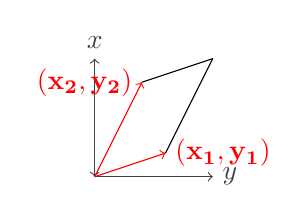
\begin{tikzpicture}[scale=.3]
\draw [<->,gray!50!black] (0,0)--(0,5) node[above]{$x$};
\draw [->,gray!50!black] (0,0)--(5,0) node[right]{$y$};

\draw [->,red] (0,0)--(2,4) node[left] {$\mathbf{(x_2,y_2)}$};
\draw [->,red] (0,0)--(3,1) node[right] {$\mathbf{(x_1,y_1)}$};

\draw [-,black] (2,4)--(5,5);
\draw [-,black] (3,1)--(5,5);
\end{tikzpicture}
\end{center}

Show that the magnitude (i.e., absolute value) of $\det(\mathbf{A})$ is equal to the area of a parallelogram formed by the column vectors of the matrix $\mathbf{A}$.
\item What is the determinant of $\mathbf{A}$ if its column vectors are on the same line? Graphically, what happens to the parallelogram?
\end{enumerate}
\end{prob}
\begin{sol}
	\begin{enumerate}
		\item \item \begin{center}
		    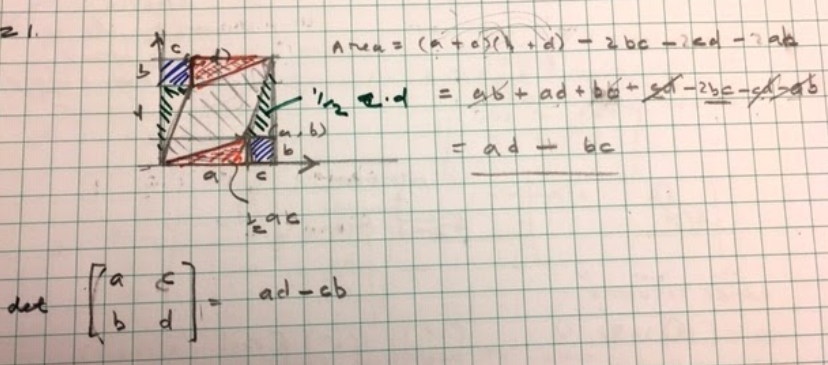
\includegraphics[scale=0.5]{FacesNight3/figs/parallelogram.png}
		\end{center}
	\item The determinant is equal to 0, or det$(\mathbf{A})$=0.
	\end{enumerate}
\end{sol}

From this, you should get the feeling for the fact that the determinant is a measure of how co-linear the columns of $\mathbf{A}$ are:  or in other words, how linearly independent the two columns are.  The determinant therefore lets us know quickly if a linear system of algebraic equations has a solution, as illustrated in the following example.

\begin{prob}
Consider the following matrix whose columns lie on the same line: the second column is simply twice the first column.
\begin{align}
\mathbf{A} = \twobytwo{1}{2}{2}{4}
\end{align}
\begin{enumerate}
\item What is det$(\mathbf{A})$?
\item Find all the solutions to $\mathbf{A} \mathbf{x} = \mathbf{0}$.
\item For which vectors $\mathbf{b}$ does $\mathbf{A} \mathbf{x} = \mathbf{b}$ have a solution? Why are there only certain $\mathbf{b}$ vectors that lead to solutions to $\mathbf{A} \mathbf{x} = \mathbf{b}$?
\end{enumerate}
\end{prob}

\begin{sol}
	\begin{enumerate}
		\item det$(\mathbf{A})$=(1)(4)-(2)(2)=0
		\item There are infinitely many solutions of the form $-x_{1}=2x_{2}$.
		\item Solutions are of the form $\mathbf{b}=\begin{bmatrix} k \\ 2k \end{bmatrix}$ where k is a constant.
	\end{enumerate}
\end{sol}

While the formula for the determinant of a $2\times 2$ matrix is quite straightforward, the procedures for computing the determinant of larger matrices is more difficult, but they are well known and well documented.  Fortunately, MATLAB has the \texttt{det} function which computes the determinant.

\section{Linear Systems of Algebraic Equations: Formulation and Definition}

In previous classes, you've encountered a bunch of exercises where you had to operate on a vector to find another vector:
\begin{align}
\mathbf{A}\mathbf{x} = \mathbf{b},
\end{align}
where $\mathbf{A}$ and $\mathbf{x}$ were known, and your job was to find $\mathbf{b}$.  While this is fun and, as you saw above in the rectangle exercise, can be useful, there is another related problem which is easily as important.  It involves the same equation, but now you know $\mathbf{A}$ and $\mathbf{b}$ and need to find the vector $\mathbf{x}$.  As we will discuss here, this problem captures the concept of a Linear System of Algebraic Equations.

One key idea in building models is the step of abstraction: going from some real-world situation to an abstracted model for the system (e.g., a set of differential equations).  There are two important aspects of building such a model: first, deciding what to include or ignore, and second, deciding how to mathematically represent those things you choose to include.

One particularly common kind of mathematical framing is a set of linear algebraic equations, which can be represented by a matrix equation.  A general system of $m$ linear algebraic equations in $n$ unknown variables $x_1, x_2, \ldots, x_n$ takes the form
\begin{eqnarray*}
a_{11}x_1 + a_{12}x_2 + a_{13}x_3 + \ldots + a_{1n}x_n &=& b_1 \\
a_{21}x_1 + a_{22}x_2 + a_{23}x_3 + \ldots + a_{2n}x_n &=& b_2 \\
\ldots &=& \ldots \\
a_{m1}x_1 + a_{m2}x_2 + a_{m3}x_3 + \ldots + a_{mn}x_n &=& b_m
\end{eqnarray*}
where $a_{11}, a_{12}, \ldots, a_{mn}$ are known as coefficients and $b_1, b_2, b_3, \ldots, b_m$ are constants. We can write this using matrices and vectors in the form
\[ \mathbf{A} \mathbf{x} = \mathbf{b} \]
where $\mathbf{A}$ is the $m \times n$ \textit{ coefficient matrix}, $\mathbf{x}$ is the $n \times 1$ unknown vector, and $\mathbf{b}$ is a $m \times 1$ constant vector which is known. In other words,
$$\mathbf{A} = \begin{bmatrix} a_{11} & a_{12} & \cdots & a_{1n} \\ \vdots & \vdots & \ddots & \vdots \\
a_{m1} & a_{m2} & \cdots & a_{mn} \end{bmatrix} \ \mathbf{x} = \begin{bmatrix} x_1 \\ x_2 \\ \vdots \\ x_n\end{bmatrix} \ \mathbf{b} = \begin{bmatrix} b_1 \\ b_2 \\ \vdots \\ b_m \end{bmatrix}.$$

Note that ``linear'' here means linear in terms of the unknown variables, e.g., if x is an unknown there are only terms like $ax$, and no terms like $\sin(x)$, $x^2$, $1/x$, etc.  It is often the case that you might have \textit{ coefficients} that appear to be non-linear; for example, in solving physics problems, you might have coefficients that depended on trig functions of angles, such as $(L \cos \theta) F_x$, which is is linear in $F_x$ but not linear in $\theta$).  Be careful to be clear about what you're solving for when you decide whether something is linear or non-linear.

\section{Using Matrix Inverses to Solve Linear Systems}
Over the last week, you have worked with rotation matrices, and transformations that were compositions of simpler rotations, and learned how to invert them. When you multiply a vector by any matrix (not just ones that are associated with simple spatial transformations), you transform the original vector $ \mathbf{x} $ into a new vector $ \mathbf{b} $.

\[ \mathbf{A} \mathbf{x} = \mathbf{b} \]

More generally (than rotations), you can \emph{often} undo the linear transformation (just like you did with the rotation matrix). Undoing this linear transformation is a linear transformation itself! Therefore the act of undoing a linear transformation can be formulated with a matrix multiply.\\

\[ \mathbf{A}^{-1} \mathbf{A} \mathbf{x} = \mathbf{A}^{-1}\mathbf{b} \]
\[\Rightarrow \mathbf{x} = \mathbf{A}^{-1}\mathbf{b} \]

This reduces our linear system of algebraic equations problem to the problem of finding the inverse of our matrix $ \mathbf{A}$.  Note this is only possible if $\mathbf{A}$ is square and \emph{invertible}.


When solving a system of equations, at least half of the battle is typically getting your system abstracted to the point that it can be thought of as a system of linear equations. The following are a set of problems.  You don't need to solve these problems -- you just need to formulate them as linear algebra problems.




\subsection{An Investment Example}
In this section we will focus on deciding whether and how you can abstract the system to a mathematical model that can be written as a matrix equation.

\begin{prob}
Suppose that the following table describes the stock holdings of three of the QEA instructors. Also suppose that on a given day the value of the Apple, IBM and General Mill's stock are \$100, \$50 and \$20 respectively.
\vspace{0.5cm}\\
\begin{center}
\begin{tabular}{|c|c|c|c|}
  \hline
     & Apple & IBM & General Mills \\
 \hline
  Jeff & 100 & 100 & 100 \\
  Emily & 100 & 200 & 0 \\
  John & 50 & 50 & 200 \\
  \hline
\end{tabular}
\end{center}

\begin{enumerate}
\item \textit{Here's your first linear algebra formulation question:} What is the total value of the holdings for each professor on the day in question?  Can you formulate this as a matrix expression?  If so, what is it? If not, why not?

\item Now, suppose that you do not know how many shares of each stock are owned by the instructors. However, you know that the total value of the stocks for each instructor for three consecutive days is as given in the following table

\begin{center}
    \begin{tabular}{|c|c|c|c|}
    \hline
        & Jeff & Emily & John \\
        \hline
        Day 1 & \$1500 & \$2600 & \$950 \\
        Day 2 & \$1600 & \$2810 & \$1020 \\
        Day 3 & \$1400 & \$2550 & \$1000 \\
        \hline
    \end{tabular}
\end{center}

You also know that  the price of each stock on each of the three days was as follows:
\begin{center}
    \begin{tabular}{|c|c|c|c|}
    \hline
    & Apple & IBM & General Mills\\
    \hline
    Day 1 & \$100 & \$50 & \$20 \\
    Day 2 & \$110 & \$50 & \$22 \\
    Day 3 & \$100 & \$40 & \$30 \\
    \hline
    \end{tabular}
\end{center}

\textit{Now here's the second formulation question:} how many stocks of each company does each professor own?  Can you formulate this as a matrix equation?  If so, what are the matrices/vectors? If not, why not?

\end{enumerate}
\end{prob}

\begin{sol}
	\begin{enumerate}
		\item This can be formulated as $\mathbf{A}\mathbf{x}=\mathbf{b}$ where $$\mathbf{A}=\begin{bmatrix}100 & 100 & 100 \\
			100 & 200 & 0 \\
			50 & 50 & 200 \\
			\end{bmatrix}, \ \mathbf{x}=\begin{bmatrix}100 \\ 50 \\ 20\end{bmatrix}, \text{ and } \mathbf{b} = \begin{bmatrix} d_{jd} \\ d_{et} \\ d_{jg}\end{bmatrix}.$$
			Doing the matrix multiplication shows that Jeff has $d_{jd}=17000$, Emily has $d_{et}=20000$, and John has $d_{jg}=11500$. 
			
		\item There are several ways to do this. Perhaps the simplest is to compute each person's stock holding individually. To do this, we let $\mathbf{A}$ be a matrix with the stock prices
		$$\mathbf{A} = \begin{bmatrix} 100 & 50 & 20 \\ 110 & 50 & 22 \\ 100 & 40 & 30 \end{bmatrix},$$
		let $\mathbf{b}_{jd}$ be a vector representing the value of Jeff's stocks on each day,
		$$\mathbf{b}_{jd} = \begin{bmatrix} 1500 \\ 1600 \\ 1400 \end{bmatrix},$$
		and let $\mathbf{x}_{jd}$ be a vector representing Jeff's stock holdings (i.e., the first entry tells us how many stocks of Apple he has, the second entry is IBM, and the third is General Mills). This gives the equation $\mathbf{Ax}_{jd} = \mathbf{b}_{jd}$. By inverting $A$ we can solve for $\mathbf{x}_{jd}$. Then we repeat this procedure for each of the other instructors.
		
		But... we can do it quicker! Form a $3 \times 3$ matrix $\mathbf{X}$ whose columns are made the vectors $\mathbf{x}_{jd}, \mathbf{x}_{et},$ and $\mathbf{x}_{jg}$. Then form a $3 \times 3$ matrix $\mathbf{B}$ whose columns are made of the vectors $\mathbf{b}_{jd}, \mathbf{b}_{et},$ and $\mathbf{b}_{jg}$. This gives the equation $\mathbf{AX}=\mathbf{B}$. Inverting $A$, we can solve for $\mathbf{X}$:
		\begin{center}
		\begin{tabular}{|c|c|c|c|}
				\hline
				% after \\: \hline or \cline{col1-col2} \cline{col3-col4} ...
				& Jeff & Emily & John \\
				\hline
				Apple & 10 & 20 & 5 \\
				IBM & 10 & 10 & 5\\
				General Mills & 0 & 5 & 10 \\
				\hline
			\end{tabular}
		\end{center}
	\end{enumerate}
\end{sol}


\subsection{An Electrical Example}

Remembering your circuit analysis back from ISIM, recall that Kirkhoff's laws:
\begin{itemize}
\item  Kirkhoff's Voltage Law says that the sum of all the voltage drops around any loop of a circuit must sum to zero.  (Batteries contribute a voltage increase of $V$, resistors contribute a voltage drop of $IR$.)
\item Kirkhoff's Current Law says that the sum of all current going into and out of any junction of wires in the circuit must be zero.
\end{itemize}

\begin{prob}
In the following circuit, consider that there is a current $I_1$ going through resistor $R_1$, a current $I_2$ going through resistor $R_2$ and a current $I_3$ going through resistor $R_3$.  Find a linear algebra expression for the vector of our three unknown currents.
\begin{center}
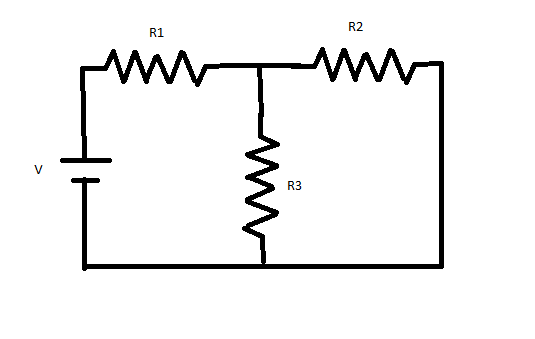
\includegraphics[width=0.75\textwidth]{FacesNight2/figs/SimpleCircuit}
\end{center}
\end{prob}

\begin{sol}
	$$\threebythree{R_{1}}{0}{R_{3}}{0}{-R_{2}}{R_{3}}{1}{-1}{-1}\threebyone{I_{1}}{I_{2}}{I_{3}}=\threebyone{v}{0}{0} $$
\end{sol}

\section{Types of Linear Systems and Types of Solutions}

Consider the linear system of algebraic equations expressed in matrix-vector form as,
\[ \mathbf{A} \mathbf{x} = \mathbf{b}. \]
If $\mathbf{b} = \mathbf{0}$ the system of linear algebraic equations is \textit{homogeneous} and if $\mathbf{b} \ne \mathbf{0}$ the system is \textit{non-homogeneous}. As mentioned before, we've already dealt with systems like this before when we were transforming geometrical objects, but in that case we already knew $\mathbf{x}$ and we were simply multiplying by $\mathbf{A}$ in order to get $\mathbf{b}$. Here, we are considering the so-called \textit{inverse} problem, and trying to find $\mathbf{x}$ given $\mathbf{A}$ and $\mathbf{b}$.
However, let's back up and consider some small examples to explore the solution possibilities a little.

\subsection{Elimination of Variables}
In high school you probably learned some basic techniques for solving small linear systems of algebraic equations. Consider the following linear system of algebraic equations,
\begin{eqnarray}
2 x_1 + 3 x_2 &=& 6 \\
4 x_1 + 9 x_2 &=& 15
\end{eqnarray}
The basic technique, called \textit{elimination of Variables}, proceeds as follows: First, solve equation (2) for $x_1$
\begin{eqnarray}
x_1 = 3 - \frac{3}{2} x_2
\end{eqnarray}
Now substitute this expression for $x_1$ into equation (3)
\[ 4 (3 - \frac{3}{2} x_2) + 9 x_2= 15 \]
Now we simplify this equation
\begin{eqnarray*}
12 - 6 x_2 + 9 x_2 &=& 15 \\
\Rightarrow 3 x_2 &=& 3
\end{eqnarray*}
and solve for $x_2$ to give $x_2 = 1$. Now we substitute this solution back into equation (2) or (4) to determine $x_1 = \frac{3}{2}$. The original linear system of algebraic equations therefore has a unique solution, $\mathbf{x} = \twobyone{1}{3/2}$.

However, not all linear systems of algebraic equations have a unique solution. For example, the system
\begin{eqnarray}
x_1 + 2 x_2 = 1 \\
2x_1 + 4 x_2 = 2
\end{eqnarray}
has an infinite number of solutions because equation (6) is just a multiple of equation (5). Solving equation (5) for $x_1$ gives
\[ x_1 = 1 - 2 x_2 \]
and choosing an arbitrary value of $x_2 = \alpha$ gives
\begin{eqnarray*}
x_1 &=& 1 - 2 \alpha \\
x_2 &=& \alpha
\end{eqnarray*}
or in vector form
\[ \mathbf{x} = \twobyone{1}{0} + \alpha \twobyone{-2}{1} \]
This defines an infinite number of solutions since $\alpha$ is any real number. What do you notice about each part of this vector?

It's also possible that a linear system of algebraic equations has no solution. For example, the system
\begin{eqnarray}
x_1 + 2 x_2 = 1 \\
2x_1 + 4 x_2 = 1
\end{eqnarray}
has no solution. Solving equation (8) for $x_2$ gives
\[ x_2 = \frac{1}{4} - \frac{1}{2} x_1 \]
and replacing into equation (7) gives
\[x_1 + 2 (\frac{1}{4} - \frac{1}{2} x_1) = 1 \]
which on simplification gives
\[ \frac{1}{2} = 1 \]
which hopefully we all agree is incorrect. We assumed that there was a solution, performed elimination and substitution and found a statement that contradicts our assumption: no solution therefore exists.

\begin{prob}
\begin{enumerate}
\item Using the technique of elimination of variables described above, determine which values of $h$ and $k$ result in the following system of linear algebraic equations having (a) no solution, (b) a unique solution, and (c) infinitely many solutions?
\begin{eqnarray*}
x_1 + h x_2 &=& 1 \\
2 x_1 + 3 x_2 &=& k
\end{eqnarray*}

\item Using the technique of elimination of variables described above, determine whether the following linear systems of algebraic equations have zero, one, or infinitely many solutions. If solution(s) exist, determine the actual solution(s).

\begin{enumerate}

\item
\begin{eqnarray*}
x_1 + x_2 + x_3 &=& 6 \\
x_2 + x_3 &=&  2 \\
x_1 - 2 x_3 &=& 4
\end{eqnarray*}

\item
\begin{eqnarray*}
x_1 + x_2 + x_3 &=& -6 \\
2x_1 + x_2 - x_3 &=&  18 \\
x_1 - 2 x_3 &=& 4
\end{eqnarray*}

\item
\begin{eqnarray*}
x_1 + x_2 + x_3 &=& 6 \\
2x_1 + x_2 - x_3 &=&  10 \\
x_1 - 2 x_3 &=& 4
\end{eqnarray*}

\end{enumerate}

\end{enumerate}
\end{prob}
\begin{sol}
	\begin{enumerate}
		\item Rearrange the equations to linear form $y=mx+b$. If the lines are identical, there are infinitely many solutions; if the lines are parallel, but don't overlap, there are zero solutions; if the lines are not parallel, there is one solution.
		\begin{enumerate}
		    \item h=3/2, k$\neq$2, 
		    \item h$\neq$3/2,
		    \item h=3/2, k=2
		\end{enumerate}
		\item \begin{enumerate}
			\item $x=\threebyone{4}{2}{0}$
			\item No Solution
			\item Infinite Solutions
		\end{enumerate}
	\end{enumerate}
\end{sol}

%\subsection{Gaussian Elimination}
%
%The basic process of \textit{ elimination of variables} can be formalized and is known as Gaussian Elimination. Here will briefly introduce it and you should consult other sources, such as the \textit{ Gaussian Elimination} page at WolframMathWorld for more details.
%
%Rather than writing equations, we can cast the linear system of algebraic equations in matrix form and perform \textit{ Gaussian Elimination} on the augmented matrix $[\mathbf{A} \; \mathbf{b}]$. For our original example we have
%\[ \twobythree{2}{3}{6}{4}{9}{15} \]
%Thinking now in terms of rows, we replace the second row with row 2 - 2 row 1 to give
%\[ \twobythree{2}{3}{6}{0}{3}{3} \]
%This matrix is now in so-called \textit{ echelon} form: we can find the solution to the original linear system of algebraic equations by first solving the equation implied by the last row and then back-substituting into the equation implied by the previous row. Unfortunately, there is no method in MATLAB that performs Gaussian Elimination in this manner.
%
%\begin{enumerate}[resume]
%\item Set up the augmented matrix for the last three examples and perform \textit{ Gaussian Elimination} to reduce the augmented matrix to \textit{ echelon form}. Interpret the resulting system and determine the solution(s).
%\end{enumerate}
%
%
%\subsection{Gauss-Jordan Elimination}
%
%Gauss-Jordan elimination is an extension of Gaussian Elimination in order to produce a matrix in \textit{ reduced row echelon form}. Here we will briefly introduce it and you should consult other sources, such as the \textit{ Gaussian Elimination} page at Wikipedia for more details.
%
%Starting with the matrix in echelon form
%\[ \twobythree{2}{3}{6}{0}{3}{3} \]
%we eliminate the entry in row 1, column 2 by replacing row 1 with row 1 - row 2
%\[ \twobythree{2}{0}{3}{0}{3}{3} \]
%Although we didn't intend it, we also obtained a 0 in row 1, column 2. If we didn't have a 0 there we would perform another row operation in order to obtain a 0 there. Finally we divide the first row by 2 and the second row by 3 to give
%\[ \twobythree{1}{0}{3/2}{0}{1}{1} \]
%This matrix is now in \textit{ reduced row echelon form} and we simply read off the solution. Fortunately, there is an algorithm in MATLAB, \textit{ rref}, which will perform Gauss-Jordan elimination for you.
%
%\begin{enumerate}[resume]
%\item Set up the augmented matrix for the last three examples and perform \textit{ Gauss-Jordan Elimination} to reduce the augmented matrix to \textit{ reduced row echelon form}. Check your answer by using \textit{ rref}. Interpret the resulting system and determine the solution(s).

\subsection{Solving a linear system of algebraic equations in MATLAB}

\begin{prob}
In the last class, you worked with an example of fruits in your refrigerator, and we asked you questions like how to calculate the total weight of the fruits, how many fruits there are, etc. We can use matrix operations to calculate \emph{inverse problems} as well, as this question illustrates. Suppose that you know that you have apples and oranges in the fridge and that in the genetically engineered future, the weights of all apples are 3oz and all oranges are 4oz. Because of inflation in this genetically engineered future, the price of each apple is \$1 and the price of each orange is \$2. Suppose that you also know that you paid \$13 total for your fruit and the total weight of the fruit is 33 oz. We can use this information and tools we have developed to figure out how many apples and oranges we have.  Let $n_o$ and $n_a$ be the numbers of oranges and apples in your fridge respectively, and that you don't know what these numbers are. Define the following vectors
    \begin{align}
    \mathbf{n} &= \twobyone{n_o}{n_a}\\
    \mathbf{d} &= \twobyone{13}{33}
    \end{align}
\begin{enumerate}
\item Write an equation relating $\mathbf{n}$ and $\mathbf{d}$, using a matrix-vector product.
\item Calculate how many oranges and apples you have.
\item Why this kind of problem is often called an inverse problem?
\end{enumerate}
\end{prob}
\begin{sol}
    \begin{enumerate}
        \item $\twobytwo{2}{1}{4}{3}\twobyone{n_{o}}{n_{a}}=\twobyone{13}{33}$
        \item $\twobyone{n_{o}}{n_{a}}=\twobyone{3}{7}$
        \item In this case we know the result $\mathbf{b}$, and are working backwards to find the number of apples and oranges. We also use a matrix inverse to find the result.
    \end{enumerate}
\end{sol}

\begin{prob}
\begin{enumerate}
\item Consider the example with the fruits that you worked out earlier. Now,  in addition to apples and oranges, suppose you also had an unknown number of pears which each weigh 3 oz, and cost \$3. Additionally, suppose that the total weight of the fruits is 45 oz, and you paid a total of \$21 for the fruit.

    \begin{enumerate}
    \item If possible find the numbers of oranges, apples and pears. If not, please explain why.
    
    \item Suppose that you additionally know that you have a total of 14 fruits. Can you formulate and solve a matrix-vector equation to find out the numbers of oranges, apples and pears you have?
    
    \item What is the determinant of the matrix you have set up to solve this?
    \end{enumerate}
    
\item The fruit vendors bought the pricing algorithm from Uber. Oranges are still \$2, pears are now only \$1.50, and (due to an influx of teachers) apples are now surging at \$1.50 each. Their weights stay the same. You return to the market, and again purchase 14 fruits, which have the same total weight and total cost.
\begin{enumerate}
	\item Can you formulate and solve a matrix-vector equation to find out the numbers of oranges, apples and pears you have?
	
    \item What is the determinant of the matrix you have set up to solve this?
 \end{enumerate}

\item Recall the example with fruits from class: Suppose that you have a total number of 14 apples, oranges and pears in your fridge. Suppose that each apple costs \$1, each orange costs \$ 2 and each pear costs \$3. Assume also that the weights of every apple is 3 oz, every orange is 4  oz and every pear is 3 oz.  Additionally, suppose that the total weight of the fruits is 45 oz, and you paid a total of \$21 for the fruit.

    \begin{enumerate}
    \item Formulate (or look up your formulation from class) and write down (but don't solve it yet) a matrix-vector equation to find out the numbers of oranges, apples and pears you have.
    
    \item Solve this equation to find the numbers of apples, oranges and pears using the following approaches (they will of course give you the same results, but we want you to get familiar with using the different operations here).
        \begin{enumerate}
        \item Using MATLAB, compute the inverse of the matrix in part a and use it to find the numbers of apples, oranges and pears.
        \item Use MATLAB's \texttt{ linsolve} function to find the  numbers of apples, oranges and pears.
        \item Use MATLAB's \texttt{ $\backslash$ } operator to find the  numbers of apples, oranges and pears.
        \end{enumerate}
    \end{enumerate}
\end{enumerate}
\end{prob}

\begin{sol}
    \begin{enumerate}
        \item \begin{enumerate}
            \item No, you have three unknowns and only two equations.
            \item Yes, you now have three equations and three unknowns. \[ \threebythree{2}{1}{3}{4}{3}{3}{1}{1}{1}\threebyone{n_{o}}{n{_a}}{n_{p}}=\threebyone{21}{45}{14} \] \[\threebyone{n_{o}}{n{_a}}{n_{p}}=\threebyone{3}{9}{2} \]
            \item $det(\mathbf{A})=2$
        \end{enumerate}
        \item \begin{enumerate}
            \item \[ \threebythree{2}{1.50}{1.50}{4}{3}{3}{1}{1}{1}\threebyone{n_{o}}{n{_a}}{n_{p}}=\threebyone{21}{45}{14} \] This forumation cannot be solved because A is not invertible.
            \item $det(\mathbf{A})=0$
        \end{enumerate}
        \item \begin{enumerate}
            \item \[ \threebythree{2}{1}{3}{4}{3}{3}{1}{1}{1}\threebyone{n_{o}}{n{_a}}{n_{p}}=\threebyone{21}{45}{14} \] 
            \item \begin{enumerate}
                \item \[\threebyone{n_{o}}{n{_a}}{n_{p}}=\threebyone{3}{9}{2} \]
                \item \[\threebyone{n_{o}}{n{_a}}{n_{p}}=\threebyone{3}{9}{2} \]
                \item \[\threebyone{n_{o}}{n{_a}}{n_{p}}=\threebyone{3}{9}{2} \]
            \end{enumerate}
        \end{enumerate}
    \end{enumerate}
\end{sol}

\section{Conceptual Quiz}

\begin{enumerate}
    \item Select the matrices which are invertible.
    \begin{enumerate}
        \item \twobytwo{2}{3}{1}{4}
        \item \twobytwo{1}{0}{1}{0}
        \item \twobytwo{0}{0}{0}{0}
        \item \twobytwo{1}{2}{4}{8}
        \item \twobytwo{\frac{1}{\sqrt{2}}}{\frac{1}{\sqrt{2}}}{\frac{1}{\sqrt{2}}}{\frac{1}{\sqrt{2}}}
    \end{enumerate}
    
    \item Let $(a,b,c)$ be the point of interesection for the following three planes, pictured below:
    $$z = 2 -x -y$$
    $$z = (31-6x+4y)/5$$
    $$z = (13 - 5x - 2y)/2$$
    \begin{center}
        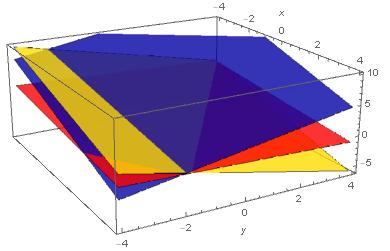
\includegraphics[scale=0.7]{FacesNight3/figs/planes.jpg}
    \end{center}
    What is $a$?
    
    \item How many solutions does the following system of equations have?
    $$x+y=9$$
    $$x-z = 2$$
    $$y+z=7$$
    A. Zero\\
    B. One\\
    C. Two\\
    D. Infinitely many
    
    \item What is the area of a parallelogram whose vertices are $(0,0)$, $(2,4)$, $(5,1)$ and $(7,5)$?
    
    \item Solve the following system of linear equations
    $$x-y=2$$
    $$3x+z=11$$
    $$y-2z=-3$$
    What is the value of $y$?
    
\end{enumerate}

\pagebreak
\shipoutAnswer